
\chapter{CPU simulation using interpretation}

The CPU simulators using interpretation are more akin to the functional simulators, as in, they directly implement
functional characteristics in the simulator code, without any translation layers. This chapter aims to provide a
general overview of the mechanisms used in such simulators and compare the general concepts with the translation
simulators. Because of their inherent simplicity, this chapter will be much shorter than the previous one.

Code snippets from the Dromajo RISC-V CPU simulator will be provided to support the explanations. This document will not
cover Dromajo's implementation of machine simulation instead will focus mainly on the CPU simulation aspect.

\section*{Interpretation simulator fundamentals}

Since the code doesn't need to be translated, the simulator directly executes the loaded binary. As is the case with
QEMU and Renode Tlib's, Dromajo also implements a virtual memory management unit, although this implementation is too
very simplified, implementing only \texttt{sv39} and \texttt{sv48} page based, virtual-memory systems \cite{RISC-PRIV}.

After the code has been loaded, and the program counter has been set to the correct value, the interpretation method
can be called. In the case of the Dromajo, the method starting the execution is \texttt{riscv\_cpu\_interp()}, which
then calls the \texttt{riscv\_cpu\_interp64()}, defined in the \texttt{dromajo\_template.h} file. The simulator then
enters the main execution loop, which checks for the interrupts, TLB status, and finally proceeds to interpret the code.

\section{Code interpretation}

The code interpretation is a step equivalent to the TCG Frontend, described in the section \ref{sec:tcg-frontend}.
Loaded instruction is separated into an opcode and operands. After that, the simulator interprets the instruction
and executes it by modifying the internal CPU state.

The lack of a translation process is a key characteristic that distinguishes interpretation CPU simulators from their
translation counterparts, and is one of the main arguments in favor of using interpretation simulators, as they
are inherently portable. They do not require guest to host or intermediate representation to host translators, witch
means that they can be used under any architecture they can be compiled for.

Since Dromajo is written in \texttt{C++} and uses \texttt{Cmake} as a build system, it can be run on most, if not all,
of the current operating systems and architectures.

\pagebreak

\section{Code execution}

The code execution takes place in the main execution loop, a concept similar to the QEMU main execution loop.

\begin{lstlisting}[
    style=lstC,
    label={lst:dromajo-interpret},
    caption={The Dromajo instruction interpretation.}
    ]
int no_inline glue(riscv_cpu_interp, XLEN)(RISCVCPUState *s, int n_cycles) {
    for (;;) {
    ...
    opcode = insn & 0x7f;
    rd     = (insn >> 7) & 0x1f;
    rs1    = (insn >> 15) & 0x1f;
    rs2    = (insn >> 20) & 0x1f;
    switch (opcode) {
        ...
        case 0x37: /* lui */
                if (rd != 0)
                    write_reg(rd, (int32_t)(insn & 0xfffff000));
                NEXT_INSN;
        case 0x17: /* auipc */
            if (rd != 0)
                write_reg(rd, (intx_t)(GET_PC() + (int32_t)(insn & 0xfffff000)));
            NEXT_INSN;
        ...
    }
\end{lstlisting}

\noindent
This \texttt{switch/case} block contains all of the supported instructions. After executing the instruction, the code
executes \texttt{NEXT\_INSN} macro, which expands to \texttt{code\_ptr += 4; break}, incrementing the code pointer, and
exiting the switch block, and returning to the beginning of the main loop. This process is then repeated indefinitely,
until an exception or an interrupt has been raised, or the simulator had finished executing the requested amount of
instructions.

\section{Exception and interrupt handling}

Similar to the case of QEMU and Tlib, both the exceptions and interrupts are handled by the same function, with the only
the difference being the way they are generated.

\subsection*{Exception Generating}

An exception can be triggered for example upon execution of trap raising instruction, such as \texttt{ecall}:

\begin{lstlisting}[
    style=lstC,
    label={lst:dromajo-generate-exception},
    caption={Generating an exception in Dromajo.}
    ]
case 0x000: /* ecall */
    if (insn & 0x000fff80)
        goto illegal_insn;
    s->pending_exception = CAUSE_USER_ECALL + s->priv;
    s->pending_tval      = 0;
    goto exception;
\end{lstlisting}

\pagebreak

\noindent
The \texttt{illegal\_insn} and \texttt{exception} labels are found after the end of the main execution loop:

\begin{lstlisting}[
    style=lstC,
    label={lst:dromajo-enter-exception},
    caption={Entering the exception handler in Dromajo.}
    ]
illegal_insn:
    s->pending_exception = CAUSE_ILLEGAL_INSTRUCTION;
    s->pending_tval      = 0;
mmu_exception:
exception:
    ...
    raise_exception2(s, s->pending_exception, s->pending_tval);
\end{lstlisting}

\subsection*{Interrupt generating}

Interrupts requests are checked and generated at the very top of the execution loop:

\begin{lstlisting}[
    style=lstC,
    label={lst:dromajo-generate-interrupt},
    caption={Generating an interrupt in Dromajo.}
    ]
...
/* check pending interrupts */
if (unlikely(((s->mip & s->mie) != 0) && ...)) {
    if (raise_interrupt(s)) {
        goto the_end;
    }
}
...

static int __must_use_result raise_interrupt(RISCVCPUState *s) {
    mask = get_pending_irq_mask(s);

    raise_exception(s, irq_num | CAUSE_INTERRUPT);
    return -1;
}

static inline uint32_t get_pending_irq_mask(RISCVCPUState *s) {
    pending_ints = s->mip & s->mie;
    /* Determine what IRQ's are enabled */
    ...
    return pending_ints & enabled_ints;
}
\end{lstlisting}

\noindent
At the end of the \texttt{raise\_interrupt()} function is called, invoking the same flow as for the exception.

\section*{Handling the exceptions}

Exception and interrupt handling is done in the \texttt{raise\_interrupt()} function, which is an implementation of
a RISC-V excetpion handling model. This method determines if the event is an IRQ or an internal CPU trap, handles
delegating the event to the lower privilege modes, etc.

\pagebreak

\section{Interpretation CPU simulator flow}

The flow will be presented based on the Dromajo simulator, but it is generally a common approach.

% image here showing the TCG layers
\begin{figure}[h]
	\centering
	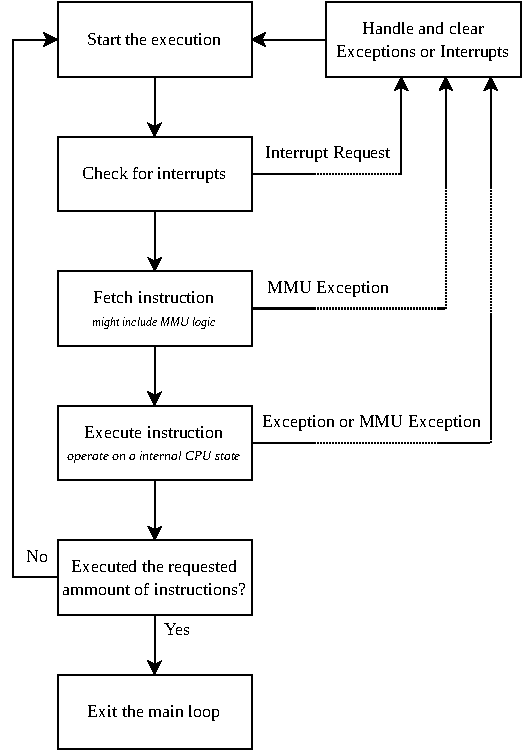
\includegraphics[width=0.75\textwidth]{figures/DromajoFlow.pdf}
	\caption{Interpretation CPU flow}
\end{figure}

\noindent
The flow is much simpler than the one QEMU implements, described in the previous chapter. Keeping in mind the general
simulator constraints mentioned in the second chapter, it should be clear that such simplicity comes at the cost of
performance. An analysis how much performance is lost due to the lack of optimizations that translation CPU simulators
implement is the main point of this work and will be conducted in Chapter 5.